\subsection{Método de desarrollo}

El proyecto se desarrollará mediante un sistema de fases, en las que el orden es algo vital puesto que cada una de las fases dependerá de la previa, en la \acrfull{edt} (figura \ref{fig:edt}) puede verse su estructura.

\begin{figure}[!htp]
	\centering
	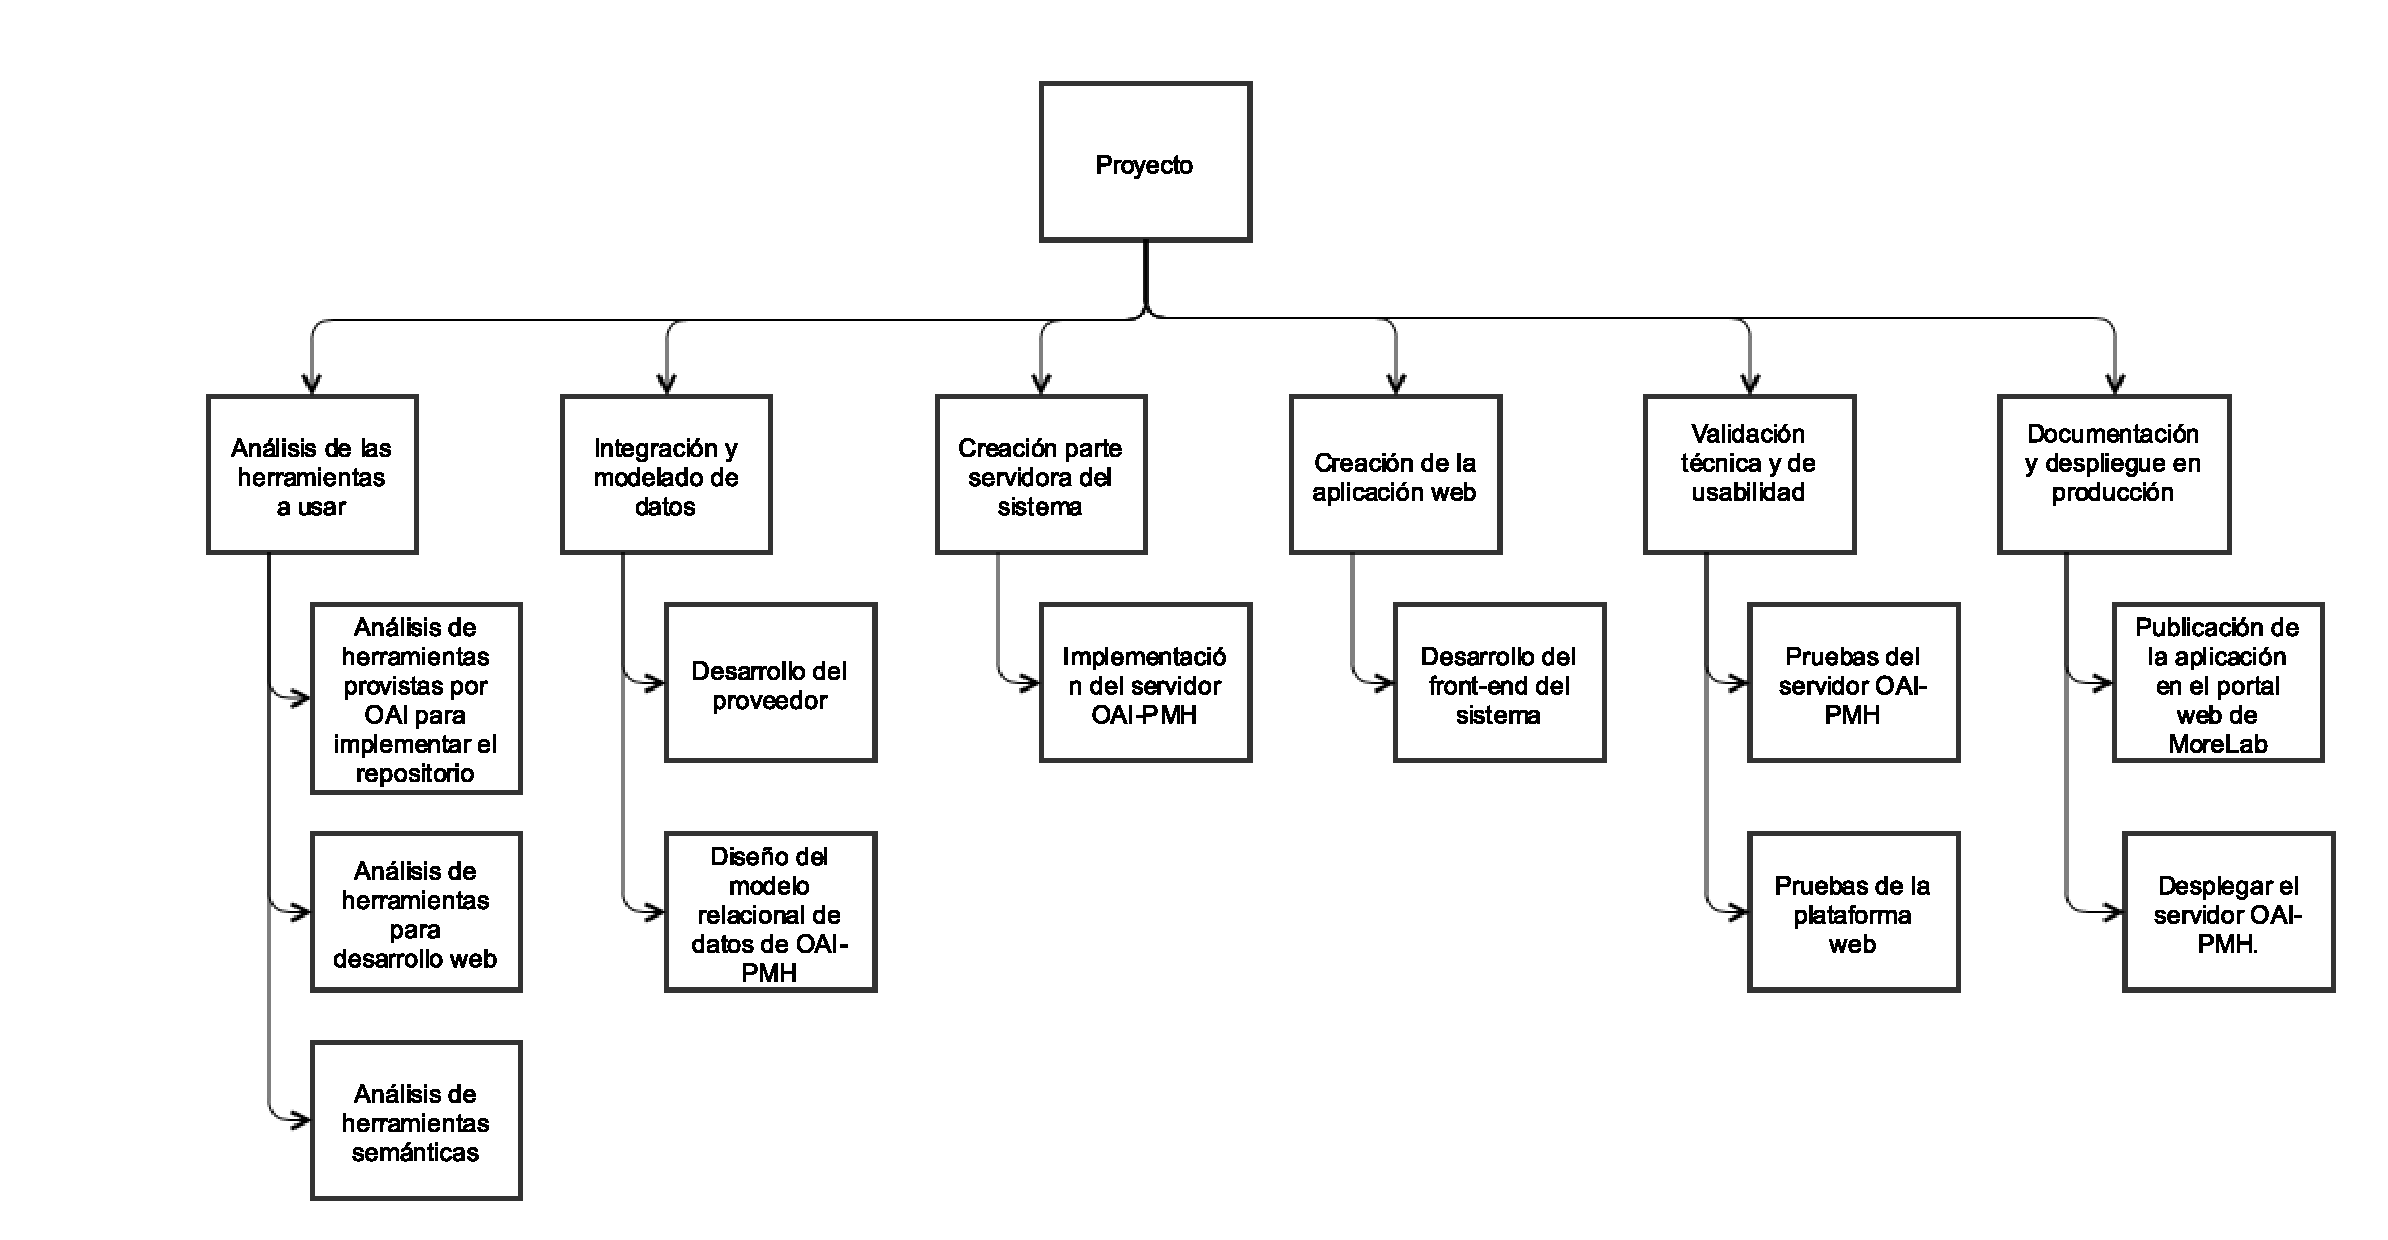
\includegraphics[angle=90, scale=.5]{fig/edt}
	\caption{EDT}\label{fig:edt}
\end{figure}

Por tanto, las fases de la solución planteada serán las siguientes:

\begin{enumerate}
	\item \textbf{Análisis de las herramientas a usar:}

	En esta fase se analizarán todas las posibles herramientas que se pueden usar para el desarrollo del proyecto, se elegirán las más adecuadas de acuerdo a las necesidades del mismo y a los conocimientos del equipo de trabajo.
	\item \textbf{Integración y modelado de datos:}

	Es la fase en la que se identificarán y seleccionarán las tablas del repositorio de las que se extraerá la información para su adaptación a Dublin Core.
	\item \textbf{Creación del servidor de OAI-PMH:}

	Diseño e implementación del servidor.
	\item \textbf{Creación de la aplicación web:}

	Diseño e implementación del front-end de la aplicación web. 
	\item \textbf{Validación técnica y de usabilidad:}

	Es la fase donde se realizarán las pruebas finales del sistema completo.
	\item \textbf{Documentación y despliegue en producción:}

	Es donde se terminará de redactar la documentación necesaria y se desplegará el producto.
\end{enumerate}